\chapter[Literature review]{Literature review }
\label{Chap:label}	%CREATE YOUR OWN LABEL.
\pagestyle{headings}



Some of the concepts behind the proposed project, such as an Ethernet MAC or RISC-V processor are not new. Consequently, there is a variety of previous work 
in these areas. This part of the proposal will explore the prior work related to the project. 


\section{Field Programmable Gate Arrays}
\label{subsection:fpga}	
First introduced by Xilinx in 1984, field programmable gate arrays (FPGAs) allowed for large custom logic designs to be recognised without the need for 
expensive application specific integrated circuits (ASICs). More importantly, FPGAs did not suffer from the same scalability issues that
programmable array logic (PAL) encountered and has allowed for larger and more complex designs \cite{30YearsOfFPGA}. 

A big advantage to custom logic is the ability to create highly parallelised designs with lower latencies than software based serialised algorithms. This comes down to 
having a great degree of freedom when it comes to designing the architecture and ability to optimise for specific tasks.
As such, FPGAs have became ubiquitous in both digital signal processing and for accelerating an assortment of heterogeneous computing architectures and processes \cite{FPGAComputing}.
System on chip (SoC) design with custom hardware acceleration modules is an active area research. As \cite{FPGAComputing} points out, there is a focus towards 
using both hardware and software in \textit{edge} devices due to growing numbers of IoT devices.


Several papers, \cite{LwIPFPGAFirewall} \cite{IPFPGAFirewall2000} \cite{packetFilteringFPGA}, have proposed a range of other related FPGA based firewalls that have 
different properties and focus on different optimisations. The key benefit to these firewalls is their high performance - namely, low latency, and high throughput. 
Article \cite{LwIPFPGAFirewall} proposed an Ethernet firewall using LwIP (A TCP/IP stack) with five-tuple binding (the five filtered parameters in packet filters) 
to achieve a throughput of 950Mbps with a latency of 61.266us. A conference proceeding in 2000 \cite{IPFPGAFirewall2000} used a comparator unit to check the 
fields of the IP headers obtained a filtering rate of 500,000 packets per second. 


The enabling concept behind the above FPGA based firewalls is SoC design which involves integrating multiple components into a single package, or in this case a 
single FPGA. Often these will include small softcore microprocessors and some custom hardware such as the Ethernet or packet filtering like the proposed packet filters in \cite{LwIPFPGAFirewall}.
Having a microprocessor in the FPGA design can significantly reduce the complexity of the design and allows for quick and easy development in software instead of 
hardware \cite{SoftcoreBasedEmbeddedSystems}. In FPGA design, softcore processors are configurable and can be modelled in a hardware description language (HDL) 
which can then be synthesised onto ASICs or FPGAs hardware \cite{SoftcoreBasedEmbeddedSystems}. There are several softcore processors available for FPGA 
designs including ARM Cortex, Nios II, MicroBlaze, and RISC-V. 
 
While recently the royalty free RISC-V based cores have been popular amongst many SoC designs, other older processors are still common in the literature. The two 
big FPGA vendors, Xilinx (now AMD) and Altera (now Intel) have their own RISC based softcores. As an example, Janik et al. \cite{LwIPMicroblaze} used Xilinx's MicroBlaze processor 
as a media converter between optical (SFP interface) and copper (Ethernet) networks. Likewise, Altera's Nios II can be found in a variety of research papers 
including an embedded web server which significantly simplified the design \cite{NiosIIWebserver}. 



\section{Packet Filter Firewall}

Usually, the first line of defence against bad actors, firewalls play a vital component in computer networks and as such can become vastly complex. 
In essence, the job of a firewall is to isolate and restrict access to an internal network from an external one to increase security \cite{BuildingInternetFirewalls}.

There are several types of firewalls such as packet filters (PF), stateful packet firewalls and application firewalls \cite{FirewallsBook}. 
Traditional PFs are considered as stateless and filter exclusively on the fields in the network (layer 2) and transport 
(layer 3) layer headers \cite{FirewallsBook}. Such fields include IP addresses, port numbers and protocol type.

Due to this, PFs are inherently simple and efficient. Consequently, they are widely available and can be either implemented in software or in 
hardware \cite{BuildingInternetFirewalls}. The book, \cite{BuildingInternetFirewalls}, also highlights some inherent flaws with PFs which include not being able 
to suppress sophisticated attacks and in some cases, can be challenging to properly configure. More advanced firewalls can perform deep packet inspection which 
explore the contents of the higher layers to better evaluate a packets true intention \cite{FirewallsBook}. 

While firewalls such as \textit{iptables} in Linux are software based, hardware acceleration can vastly improve the performance of a packet filter. As stated in section 
\ref{subsection:fpga}, hardware acceleration allows for parallelised algorithms to be executed independently of a central processing unit (CPU). Wicaksana and Sasongko, 
\cite{FastRecongifFPGAFirewall}, proposed a packet classification engine as shown in figure \ref{fig:fast-fpga-classifier}. To obtain a fast and reconfigurable packet 
classifier, the authors of \cite{FastRecongifFPGAFirewall} used a hierarchical tree-based algorithm that inspects the multidimensional fields of the IP header through 
the use of parallel decision trees.

Essentially, the architecture in figure \ref{fig:fast-fpga-classifier} employs memory to store the ruleset and uses a multiplexer and a comparator to evaluate each of the fields 
in the header. As an safegaurd, the authors opted for a \textit{default-deny} ruleset to prevent any unwanted traffic. 


\begin{figure}[h]
    \centering
    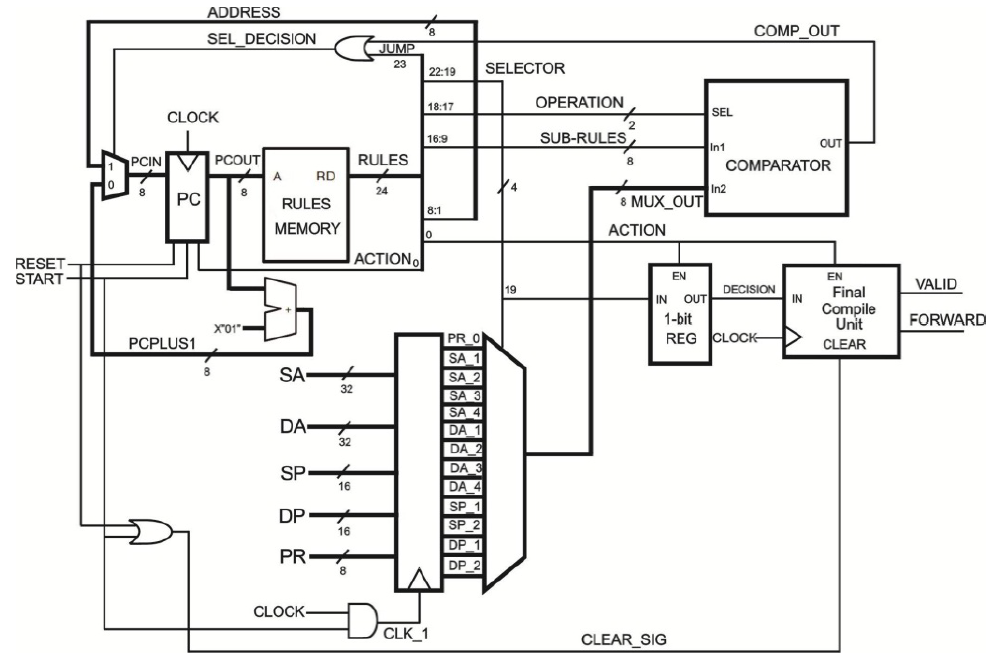
\includegraphics[width=0.8\textwidth]{Images/packetFilterHardware.png}
    \caption{Packet classifier \cite{FastRecongifFPGAFirewall}}
    \label{fig:fast-fpga-classifier}
\end{figure}


\newpage

Wasti \cite{Wasti2001HardwareAP} presents several other classification algorithms for both hardware and software packet filters. \textit{'Sequential matching'} provides the most 
trivial solution as it matches each rule to the incoming packet. While simple, this design has scalability issues as more rules get added. Another method proposed in 
\cite{Wasti2001HardwareAP} is by using a \textit{'Grid of tries'} which uses tries (a type of tree datastructure) to help pattern match the packets, but fails to extend to multiple fields. 
Hardware algorithms using \textit{Ternary CAMs} (stores words with 3-valued-digits - namely '0', '1' and '*') and \textit{Bit-parallelism} were also discussed. Both of these 
exploited the parallelised nature of hardware design. One limiting factor with the classification methods cited in \cite{Wasti2001HardwareAP} is their configurability and 
expandability. 



\section{RISC-V processor}
In the world of processor architectures, there are four major families, namely AMD64, x86, ARM and RISC-V. The two former instruction set architectures (ISA) 
are apart of the complex instructions sets (CISC) and are found in the majority of computers. ARM and RISC-V have a reduced instruction set compared to the CISC family and 
subsequently fall under the RISC family and are ideal for low power microprocessors \cite{RV16Embedded}.

RISC-V is an open and royalty free ISA and as a result, a plethora of softcore based custom implementations have been designed \cite{CatalogRISCSoftcore}. 
Consequently, there is an abundance of articles delving into RISC-V from evaluating the ISA \cite{InvestigatingRiscv} to creating multicore architectures
\cite{RiscVMulticore}. A 2019 paper, \cite{CatalogRISCSoftcore} evaluated a variety of different RISC-V softcore processors. RISC-V International have 
also published a list\footnote[1]{See: https://github.com/riscv/riscv-isa-manual/blob/master/marchid.md} of different RISC-V implementations 
that have a unique architecture ID. The majority of these are either written in a HDL for either application specific integrated circuits (ASICs) or FPGAs.
The \textit{NEORV32 RISC-V} softcore processor is written purely in vendor-agnostic VHDL and importantly has a considerable amount of documentation. 

Being a softcore processor, control is given over which modules are implemented. Some basic features of the \textit{NEORV32 RISC-V} include 
UART, SPI, and GPIO interfaces \cite{neorv32Datasheet}. The datasheet, \cite{neorv32Datasheet}, also mentions that it supports a \textit{'Wishbone b4 classic'} 
external bus interface. A Wishbone B4 (or just 'wishbone') interconnection is designed specifically to connect modular pieces of hardware together on a 
SoC into the memory mapped 32bit address space in the processor \cite{WishboneSpec}. This approach has the benefit of not needing to create custom 
instructions for the microprocessor. 


\section{Ethernet MAC}

First introduced in 1983, the IEEE 802.3 standard \cite{IEEE802.3-2012}, more commonly known by the name of 'Ethernet', defines the \textit{'Medium Access Control'} 
(MAC) protocol amongst other things for two or more devices to communicate over a network. This standard is just one part in the layered network 
models such as the OSI model or TCP/IP model, namely the network layer - layer 2. 


A core function of the Ethernet MAC is to attach the required MAC layer headers to the head and tail of the layer 3 payload to create an Ethernet packet. The fields 
in an Ethernet packet can be seen in figure \ref{fig:ieee-mac-headers}. 

\begin{figure}[h]
    \centering
    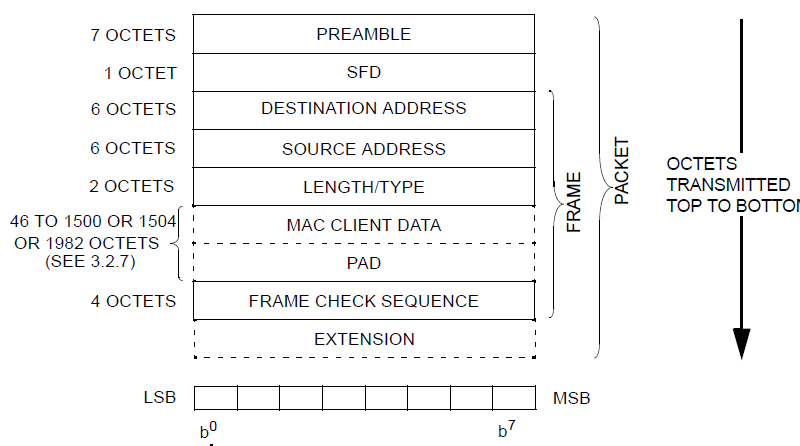
\includegraphics[width=0.65\textwidth]{Images/mac_packet.png}
    \caption{MAC layer headers \cite{IEEE802.3-2012}}
    \label{fig:ieee-mac-headers}
\end{figure}

After the packet has been constructed, the data is forwarded out to the physical (PHY) layer 
least significant bit (LSB) first \cite{IEEE802.3-2012}. Typically, a PHY management chip is used to handle the physical layer channel encoding amongst other things. 
These PHY chips often can be interfaced with the media independent interfaces such as MII, RMII, GMII and RGMII \cite{OptimisedEthernetMAC}. The reduced media 
independent interface (RMII) is one of these standards defined in \cite{IEEE802.3-2012} and consists of a reference clock, 2 bit wide transmit (TX), 2 bit wide 
receive (RX) lines and a few other supplementary signals as defined in the LAN8720A datasheet \cite{LAN8720ADatasheet}.


The MAC layer itself is usually implemented in hardware as it has several advantages over a software implementation. The core reasons behind this are due to parallelised nature of FPGAs and that parts of the MAC can operate independently \cite{reducedEtherentMacFPGA}. One key example is the calculation of the 
frame check sequence (FCS in figure \ref{fig:ieee-mac-headers}). The FCS for Ethernet is a 32bit cyclic redundancy check (CRC) \cite{IEEE802.3-2012} and 
in addition to Etherent, the CRC32 can be found in an extensive amount of applications. As such, research has been conducted into parallelising the calculation. 
Noteably, Mitra and Nayak \cite{ParallelCRC} proposed a low latency parallelised architecture for FPGA design on CRC32. As a result, packets can be assembled 
faster and offload additional processing burden from the CPU. 


Numerous articles \cite{OptimisedEthernetMAC} \cite{EthernetAXI} \cite{EthernetRMII} can be found about Ethernet MACs implemented 
on FPGAs each with a slightly different approach. Fundamentally though, as best highlighted in \cite{OptimisedEthernetMAC}, a simple way of implementing a MAC is by employing a finite state 
machine (FSM) to set the required fields. Another technique found in these articles is the use first-in first-out (FIFO) buffers to cross clock domains. This is a common technique used 
in FPGA design as it allows you to have the packet assembly logic at a much higher clock rate than the output RMII reference clock speed \cite{EthernetAXI}. 

In addition to the papers, there are a plethora of intellectual property (IP) blocks for xMII interfaces in HDL 
which have their own benefits and drawbacks. Some freely available HDL modules for Ethernet MACs can be found in both a complete \footnote[1]{See: https://github.com/yol/ethernet\_mac} \footnote[2]{See: https://github.com/alexforencich/verilog-ethernet/} 
\footnote[3]{See: https://opencores.org/projects/ethernet\_tri\_mode} and incomplete state
\footnote[4]{See: https://github.com/pabennett/ethernet\_mac}.






\section{Web servers and network stacks}

Almost all firewalls need to be configured with a ruleset which can be configured in two common ways, using a command line interface (CLI) 
or by a web-based graphical user interface (GUI). Before a web server can be realised, the network stack (Layers 3, and 4) need to be established since a web server 
operates at the application layer (layer 4). As embedded platforms are resource limited, special precautions need to be taken into consideration when it comes to memory and resource 
usage \cite{OptimCortexLwIP}.

Article \cite{LwIPFPGAFirewall} investigated using the open source lightweight IP (LwIP) network stack as a mechanism for interfacing with the firewall. 
The LwIP library is a popular lightweight TCP/IP stack which has been investigated in a plethora of research papers and projects \cite{ImprovemntOptimLWIP} 
\cite{OptimCortexLwIP}. Often these papers run LwIP on real time operating systems (RTOS) such as FreeRTOS or Zephyr.

FreeRTOS is a leading RTOS for microprocessors and is distributed freely under the MIT license. As an RTOS, it provides an abstraction to the hardware that allows 
for multitasking and brings other OS-Like features to embedded systems. Several ports are available including one for RISC-V. 

FreeRTOS also provide their own TCP/IP network stack called \textit{FreeRTOS-Plus-TCP} which includes a HTTP web server example and is much newer than LwIP.
Consequently, less research can be found apart from existing documentation. The library aims to provide a threadsafe Berkley sockets API and network stack 
supporting multiple protocols such as DHCP, DNS, TCP, and UDP \cite{FreeRTOSTCP}. LwIP is not threadsafe and typically suffers from memory issues as found 
in \cite{OptimCortexLwIP}.


